\chapter{Introduction}

% Software aging: https://www.cs.drexel.edu/~yfcai/CS451/RequiredReadings/SoftwareAging.pdf
% Measuring and Monitoring Technical Debt http://ccsl.org.br/files/TD%20talk%20USP.pdf

The resources, budget and time frame of software engineering projects are often constrained.
This requires software engineers to analyse trade-offs that have to be made in order to meet deadlines and budgets.
Making decisions that are beneficial on the short term, might lead to significantly increased maintenance costs in the future.
The phenomenon of favouring short-term development goals over longer term requirements is often referred to as \emph{technical debt}.
While technical debt might not have implicit consequences on the user experience, it dramatically impacts quality and maintainability of the software.\\\\
The term technical debt was first introduced by Ward Cunningham as writing "not quite right" code in order to ship a new product or feature to market faster.
Since then, the term has gained progressively more attention in the software engineering research and the agile community.
Effective management of such debt is considered critical to achieve and maintain a high level of software quality.
In 2007, Steve McConnell created the technical debt taxonomy where he refined and expanded the definition.
He points out that some kind of engineering practices are not considered technical debt, such as deferred features, incomplete work that is not shipped and other features where one does not have to 'pay' debt for.
Martin Fowler considers technical debt more as a metaphor to use when communicating with non-technical people and introduced the technical debt quadrant in 2009.
According to his work, technical debt can be categorized in distinct types, separating issues arising from recklessness from those decisions that are made strategically. 
Figure \ref{fig:technical-debt-quadrant} presents this distinction in more detail.\\

\begin{figure}[!h]
	\centering
	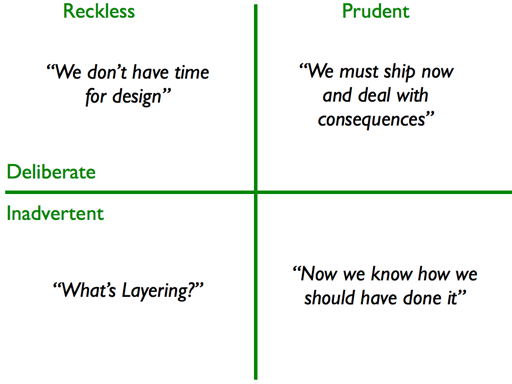
\includegraphics[width=0.5\columnwidth]{images/technical_debt_quadrant}
	\caption{The technical debt quadrant, as proposed by Martin Fowler.}
	\label{fig:technical-debt-quadrant}
\end{figure}

Technical debt can be both invisible and visible to end users.
Examples of invisible technical debt includes code smells, coding style violations, low internal quality and high code complexity.
Visible technical debt is expressed in bugs that are affecting users but can also be identified by user-unfriendly, cluttered graphical user interfaces.
Decisions to extend and evolve the graphical user interface with new visual elements, can lead to a high amount of technical debt and a poor user experience.\\\\
The term itself is borrowed from the finance domain.
There is however one important distinction between financial debt and technical debt.
When working with financial debt, the costs that the debtor has to pay is usually clear.
This is not always the case with technical debt: there might be some situations where no technical debt incurred.
For instance, if it is known for a part of the system to never be updated or maintained in the future, time can be saved by not updating the related documentation.
Software engineers have to carefully consider what technical debt they wish to incur and when this debt will be paid off.\\\\
Tribler is the result of 10 ongoing years of scientific research in the field of decentralized network technology and has incurred a serious amount of technical debt, both visible and invisible for users.
The software allows users to discover and download interesting content such as music and videos in a completely decentralized manner.
In 2014, support for anonymous download using a Tor-like protocol has been added. 
In 2015, the protocol has been extended to support for anonymous seeding of torrents.
The graphical user interface of Tribler is shown in figure \ref{fig:tribler-interface}.

\begin{figure}[!h]
	\centering
	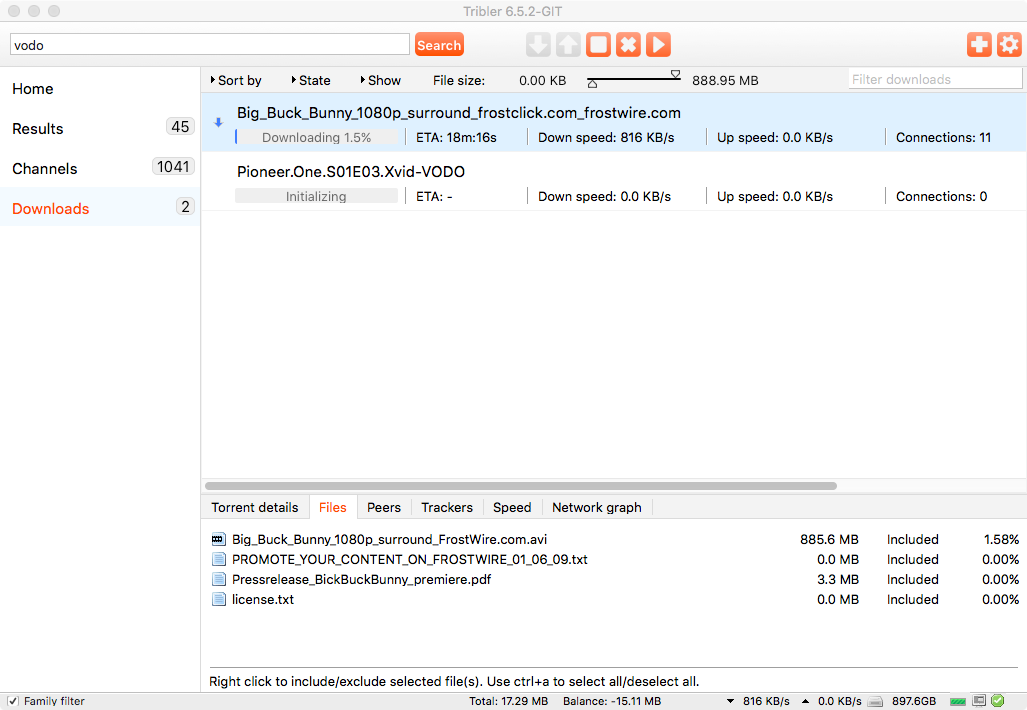
\includegraphics[width=0.9\columnwidth]{images/tribler_interface}
	\caption{The graphical user interface of Tribler v6.5.2.}
	\label{fig:tribler-interface}
\end{figure}

The focus of this thesis will be tracking and managing technical debt in Tribler. The following research question can be formulated:\\\\
\emph{How can we track and manage technical debt within Tribler?}\\\\
This question can be divided into some subquestions:
\begin{enumerate}
	\item What tools should be used to identity technical debt within Tribler?
	\item What kind of technical debt should be prioritized for fixing?
	\item What are the adequate requirements in the software development process to make the right decisions about incurring technical debt in the future?
\end{enumerate}

The rest of this document is outlined as follows: in Chapter \ref{chapter:problem-description}, the current state of the system will be elaborated, highlighting flaws and impurity in the architecture and code base. 
In Chapter \ref{chapter:architecture}, the evolution of Tribler over the past 10 years will be presented and we build foundations for the next decade of scientific research with Tribler by proposing a new future-proof and robust architecture.
Various efforts to improve quality assurance, code quality and infrastructure while paying off technical debt will be explained in Chapter \ref{chapter:refactoring}.
The performance of Tribler after refactoring efforts will be discussed in Chapter \ref{chapter:experiments}.
By conduction various benchmarks and performance measurements, the user experience of Tribler will be assessed.
We will end with the conclusions and propose future work in Chapter \ref{chapter:conclusions}.
